\documentclass[graybox]{svmult}

\usepackage{type1cm}
\usepackage{makeidx}
\usepackage{graphicx}
\usepackage{multicol}
\usepackage[bottom]{footmisc}
\usepackage{newtxtext}
\usepackage{newtxmath}

\makeindex

\begin{document}

\title*{Cybersecurity in Donated Distributed Computing for Evolutionary Algorithms}
\titlerunning{Cybersecurity in DDC for EA}

\author{Petar Tomov, Iliyan Zankinski, Todor Balabanov \textsuperscript{\tiny{0000-0003-3139-069X}}}
\authorrunning{P. Tomov et al.}
\institute{Petar Tomov \at Institute of Information and Communication Technologies - Bulgarian Academy of Sciences, acad. Georgi Bonchev Str., block 2, 1113 Sofia, Bulgaria \email{p.tomov@iit.bas.bg}
\and Iliyan Zankinski \at Institute of Information and Communication Technologies - Bulgarian Academy of Sciences, acad. Georgi Bonchev Str., block 2, 1113 Sofia, Bulgaria \email{iliyan@hsi.iccs.bas.bg}
\and Todor Balabanov \at Institute of Information and Communication Technologies - Bulgarian Academy of Sciences, acad. Georgi Bonchev Str., block 2, 1113 Sofia, Bulgaria \email{todorb@iinf.bas.bg}}
%
% Bulgarian Academy of Sciences
% Institute of Information and Communication Technologies
% acad. Georgi Bonchev Str., block 2, office 514, 1113 Sofia, Bulgaria
% http://www.iict.bas.bg/
% iict@bas.bg
%

\maketitle

\abstract*{Donated distributed computing, also known as volunteer computing, is a form of distributed computing that is organized as a public donation of calculating resources. Donated calculating power can involve thousands of separate CPUs and it can achieve the performance of a supercomputer. In most of the cases donated distributed computing is organized by open source software, which can lead to the involvement of many more volunteers. This research focuses on cybersecurity issues when donated distributed computing is used for optimization with evolutionary algorithms.}

\abstract{Donated distributed computing, also known as volunteer computing, is a form of distributed computing that is organized as a public donation of calculating resources. Donated calculating power can involve thousands of separate CPUs and it can achieve the performance of a supercomputer. In most of the cases donated distributed computing is organized by open source software, which can lead to the involvement of many more volunteers. This research focuses on cybersecurity issues when donated distributed computing is used for optimization with evolutionary algorithms.}

\section{Introduction}
\label{sec:01}

A subset of calculating problems has the characteristic that different computation steps are not strongly connected to each other and those steps can be calculated separately. In such problems, parallel programming is used and computation time is usually reduced by involving more calculating units. According to who owns and administers the calculating resources there are two groups of parallel computing - calculating devices under your own control and calculating devices under somebody else control. Part of the first group (private owned) is single machines with multi-cores or multiprocessors, supercomputer with many identical modules, a grid of identical single machines and a cluster of different single machines. It does not matter what is the hardware specification in the first group, which is common for the first group is that the organizer of the parallel computations has full access and full control over the hardware. This situation is very important when cybersecurity in massive computing is discussed. In the second group different type of computing hardware is organized to compute a common task, but calculating devices are not under the control of the person or the organization who/which is doing the computations. When the involved devices are participating in a volunteer principle there is no control of any kind over the donated calculating power. The biggest advantage of the donated distributed computing is that it comes at a very low price. The biggest disadvantage of the donated distributed computing is that it comes with a wide list of security and reliability issues. 

\begin{figure}[b]
\sidecaption
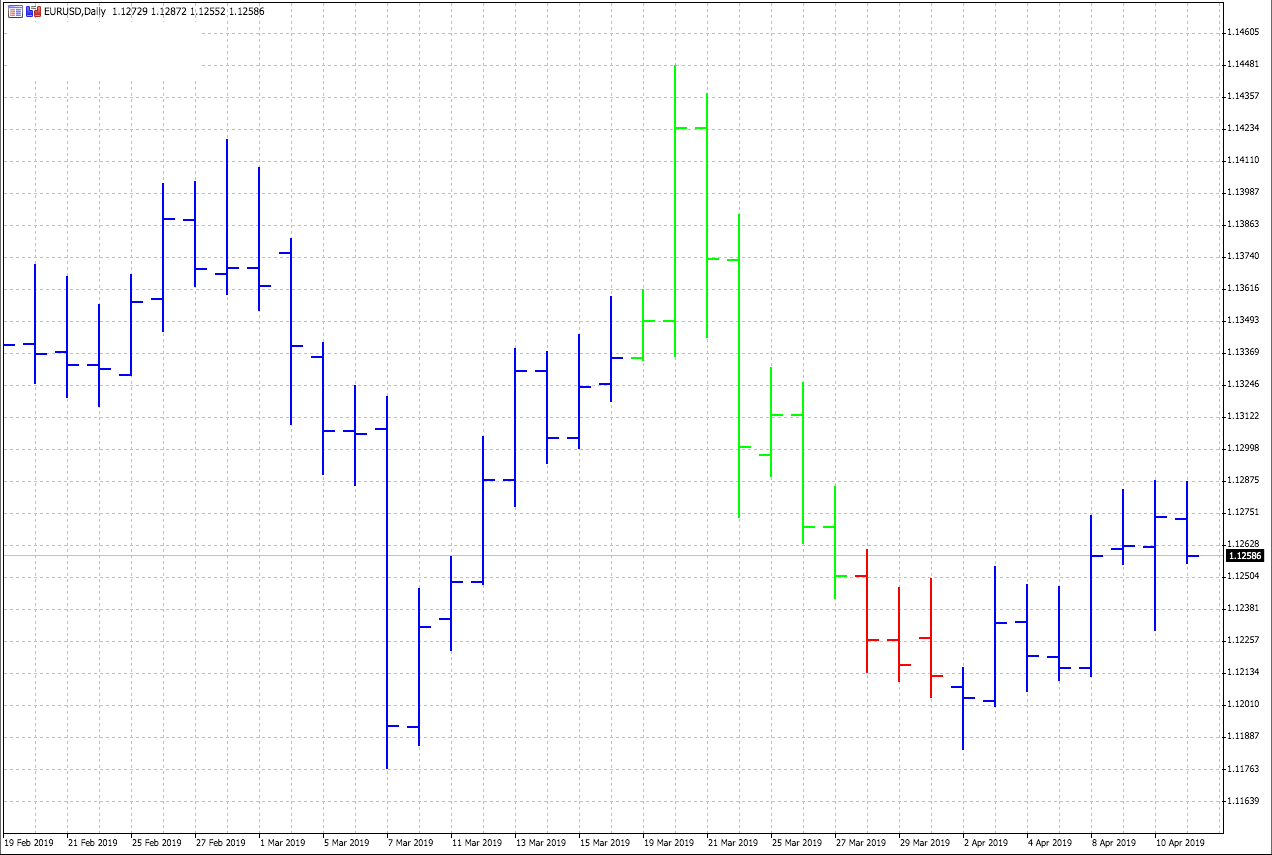
\includegraphics[width=\textwidth]{fig01}
\caption{FOREX data for EUR/USD currency pair.}
\label{fig:01}
\end{figure}

General cybersecurity does not differ in donated distributed computing than the other network communication software solutions. What is more, in donated distributed computing is related to calculation accuracy and reliability of the results. Numerical calculations that are done on different hardware can lead to different results just because of the machine word, floating-point numbers presentation and different error handling. Such differences are not human provoked and are directly math dependent. A bigger problem are human interventions with calculation instructions executed on the device and the information exchanged with the central distributed computing infrastructure. Even that it is relatively complicated a malicious user is capable to change what is calculated on his/her device directly in the device memory. A malicious user is capable to change the input data and to manipulate the output data. The general problem for the organizer of the donated distributed computing infrastructure is that he/she can not trust any of the volunteer participants. 

This study is devoted to cybersecurity issues in donated distributed computing when it is used for evolutionary algorithms. After the introductory part, the paper is organized as follows: Evolutionary algorithms in donated distributed computing are discussed; After that, some examples of damaged reliability are presented; And finally, conclusions and some further research are proposed. 

\section{Evolutionary Algorithms}
\label{sec:02}

\begin{figure}[b]
\sidecaption
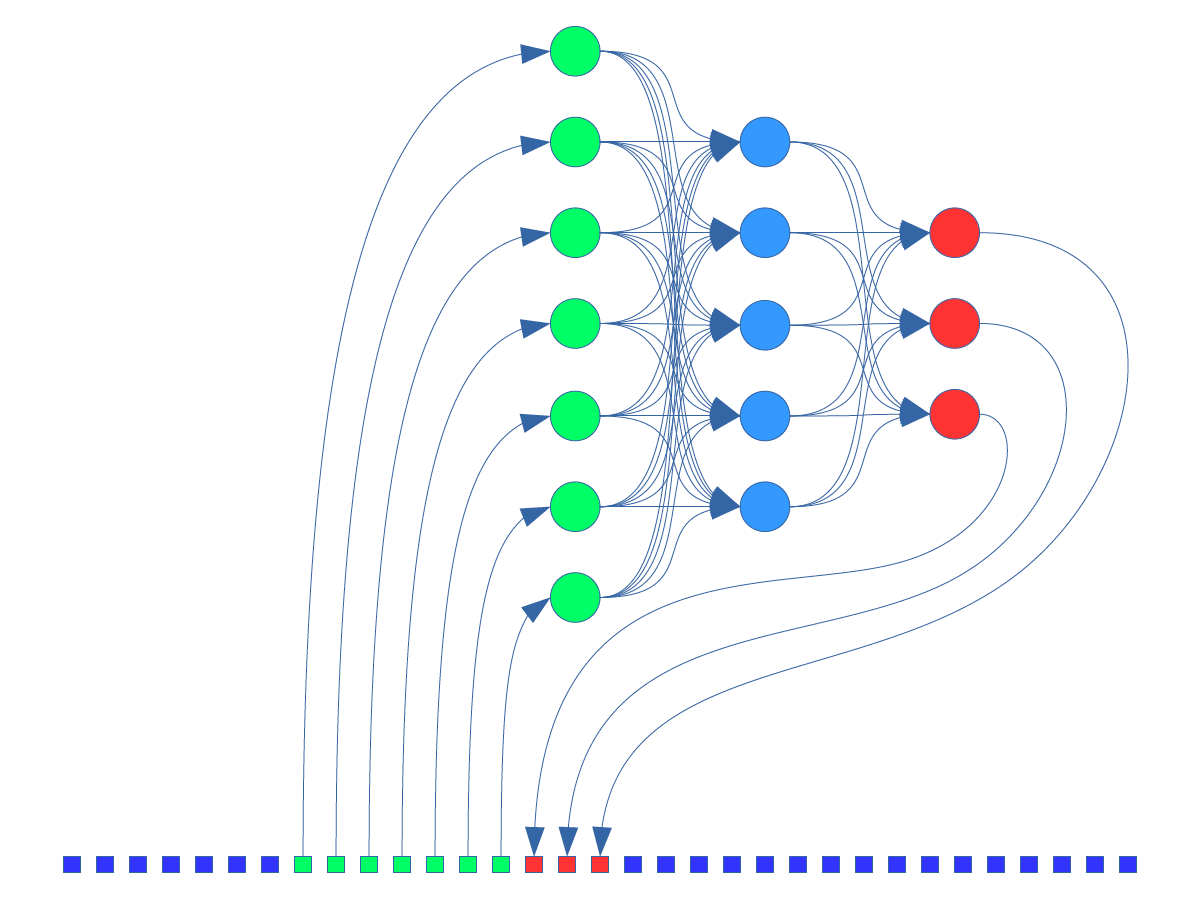
\includegraphics[width=\textwidth]{fig02}
\caption{Three-layer perceptron organized for time series forecasting.}
\label{fig:02}
\end{figure}

There are many evolutionary algorithms. The keyword in this subset of optimization algorithms is evolutionary. It means that some kind of evolution is applied. Most of the evolutionary algorithms are organized on the top of some population kind. Their application is mainly in global optimization problems. When population is used it is formed by vectors into solution space. Each individual is treated as a potential candidate for an optimal or suboptimal solution. Individuals are evaluated according predefined fitness function and the achieved fitness value is used in the process of evolution. The basic idea is that better-fitted individuals should have better chances to evolve with the hope that evolved individuals will offer better solutions. 

\begin{figure}[b]
\sidecaption
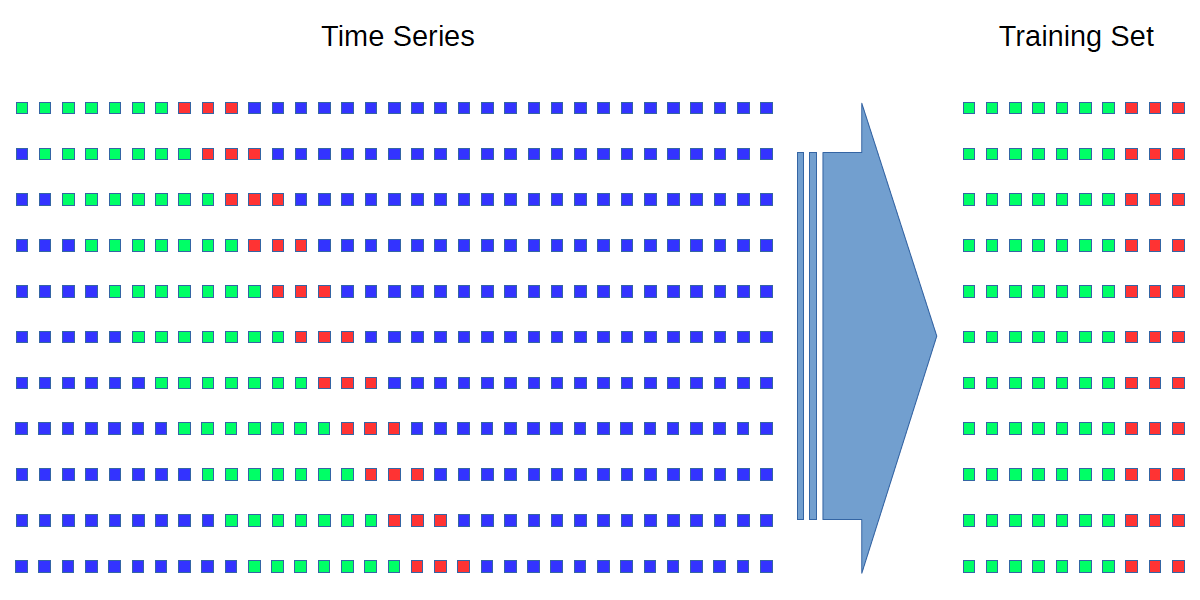
\includegraphics[width=\textwidth]{fig03}
\caption{Artificial neural network training set.}
\label{fig:03}
\end{figure}

In this research, the focus is over genetic algorithms and differential evolution used for artificial neural networks training in financial forecasting problems. Artificial neural networks are a well-known tool for classification and forecasting. Most of the artificial neural networks are organized as nodes (of neurons) and some kind of weights between the nodes. Some of the artificial neural networks are organized in layers and it is proven that with a three-layer perceptron any function can be learned. Multilayer perceptrons are used mainly with supervised training algorithms. The goal is the network to approximate a function supplied to the network with subset of input-output pairs. In this research, a three-layer perceptron is organized for financial time series forecasting (Fig. \ref{fig:02}). Time series are taken from the FOREX market (Fig. \ref{fig:01}) and present currency pairs. The data from a particular time series are conditionally organized in past values (lag) and future values (lead) (Fig. \ref{fig:03}). Past values are supplied at the input of the artificial neural network when future values are expected at the output of the artificial neural network (Fig. \ref{fig:02}). In this way each past-future pair forms a training example. Values in the training examples are scaled in the range of -0.9 and +0.9 because hyperbolic tangent is used as an activation function. Scaling is not done in the range of -1.0 and +1.0 because the extreme values are too influencing at the network input. Also, there should be a chance for the network to predict lower or higher values in the time series which were not presented yet. 

In a classical multilayer perceptron layers are fully connected. It means that each neuron has connections with all neurons from the next layer. The size of the input layer is problem dependant and it is adjusted manually or with some kind of self-adapting algorithm. The size of the output layer depends on how many values ahead are needed as a forecast. The size of the hidden layer can be set as the average of the input and output sum, but in most cases, it is experimentally adjusted. The pruning algorithm also can be used for the estimation of the hidden layer size. The topology of the artificial neural network can be put under heuristic optimization, but such an approach is not used in this research. 

\begin{figure}[b]
\sidecaption

\includegraphics[width=\textwidth]{fig04}
\caption{Mobile application for donated distributed computing in financial forecasting.}
\label{fig:04}
\end{figure}

Weights of the artificial neural network can be presented as vector of real numbers. Each vector of weights is loaded into the artificial neural network structure and it is trained with classical back-propagation until there is no prediction improvement with prespecified epsilon level. A group of weights vectors forms a local evolutionary population. The evolutionary process is applied locally and the best-found solutions are sent to the remote server in such a way that to become a part of the global population. The security problem rises exactly at this point when calculation results are sent to the remote server. There is no guarantee that what is sent is accurate and it is not manipulated by the owner of the calculating device. 

A major species of the evolutionary algorithms is that the optimization process goes across many intermediate calculations which are not used as part of the final result. If malicious user manipulates the reported results in the global population low-quality evolutionary individuals will be reported. One strategy to fight with such a cybersecurity issue in the evolutionary donated distributed computing is by checking the individual on the server-side as part of the global population. Even such a strategy is possible it is not rational and cost-efficient. The main idea of the donated computations is to lower the expenses for server operation. Keeping the cost of the calculation low on the server-side is a common goal in donated computations. Because of this, it is not preferable individuals checking to be done on the server-side. The other strategy, which is much more efficient is to keep compromised individuals as part of the global population. From one side extra server time will be kept and from another side, the checking will be done on other donated devices during the next distribution of global population subsets as local populations. By implementing aging for the individuals in the global population the compromised individuals will be removed with the time goes on. Aging also will protect server storage capacity. As an additional positive side effect, the compromised individuals act as genotype diversity into the local populations, which indirectly can work as an improvement of the evolutionary process. 

\section{Mobile Application}
\label{sec:03}

\section{Conclusions}
\label{sec:04}

\begin{acknowledgement}
This research is funded by Velbazhd Software LLC and it is partially supported by the Bulgarian Ministry of Education and Science (contract D01–205/23.11.2018) under the National Scientific Program ``Information and Communication Technologies for a Single Digital Market in Science, Education and Security (ICTinSES)'', approved by DCM \# 577/17.08.2018.
\end{acknowledgement}

\begin{thebibliography}{99.}

\bibitem{g-stock-01} Chokesatean, P.: Credibility-based Binary Feedback Model for Grid Resource Planning. University of Pittsburgh (2008)

\bibitem{mql5-cloud-network-01} Chang, C., Narayana Srirama S., Buyya, R.: Indie Fog An Efficient Fog-Computing Infrastructure for the Internet of Things. Computer \textbf{50}(9), 92--98 (2017)

\bibitem{money-bee-01} Bohn, A., Guting, T., Mansmann, T.: MoneyBee Aktienkursprognose mit kunstlicher intelligenz bei hoher rechenleistung. Wirtschaftsinf \textbf{45}, 325--333 (2003)

\bibitem{genetic-algorithms-01} Donate, J.P., Li, X., Sanchez, G.G., Miguel, A.S.: Time series forecasting by evolving artificial neural networks with genetic algorithms, differential evolution and estimation of distribution algorithm. Neural Computing and Applications \textbf{22}, 11--20 (2013)

\bibitem{time-series-01} Bandt, C., Pompe, B.: Permutation Entropy A Natural Complexity Measure for Time Series. Physical Review Letters, \textbf{88}(17), 174102 (2002)

\bibitem{time-series-02} Salvador, S., Chan, P.: Toward Accurate Dynamic Time Warping in Linear Time and Space. Intelligent Data Analysis, \textbf{11}(5) 561--580 (2007)

\bibitem{time-series-03} Lan, Y.: Computational Approaches for Time Series Analysis and Prediction Data-Driven Methods for Pseudo-Periodical Sequences. University of Bradford (2009)

\bibitem{vitosha-trade-01} Zankinski, I., Barova, M., Tomov P.: Hybrid Approach Based on Combination of Backpropagation and Evolutionary Algorithms for Artificial Neural Networks Training by Using Mobile Devices in Distributed Computing Environment. Proceedings of Large-Scale Scientific Computing, 425--432 (2018)

\bibitem{distributed-computing-01} Megiddo, N.: Applying parallel computation algorithms in the design of serial algorithms. Journal of the Association for Computing Machinery \textbf{30}(4), 852--865 (1983)

\bibitem{crowdsensing-01} Leppanen, T., Alvarez Lacasia, J., Tobe, Y., Sezaki, K., Riekki, J.: Mobile crowdsensing with mobile agents. Autonomous Agents and Multi-Agent Systems \textbf{31}, 1--35 (2017)

\bibitem{voting-01} Laukkanen, S., Kangas, A., Kangas, J.: Applying voting theory in natural resource management A case of multiple-criteria group decision support, Journal of Environmental Management, \textbf{64}(2), 127--137 (2002)

\end{thebibliography}


\end{document}
